\section{Date: 2026-10-19}
\noindent \textbf{Series ID: G17MVSFWLTRUCKS} 

\noindent This series is titled Weekday-Basis Seasonal Factors: Light Truck Production and has a frequency of Monthly. The units are Seasonal Factor and the seasonal adjustment is Not Seasonally Adjusted.The observation start date is 1996-01-01 and the observation end date is 2027-09-01.The popularity of this series is 1. \\ 

\noindent \textbf{Series ID: IY3314} 

\noindent This series is titled Export Price Index (NAICS): Nonferrous Metal (Except Aluminum) Production and Processing and has a frequency of Monthly. The units are Index Dec 2005=100 and the seasonal adjustment is Not Seasonally Adjusted.The observation start date is 2005-12-01 and the observation end date is 2026-09-01.The popularity of this series is 1. \\ 

\subsection{Raw Regression}
\noindent Regresses the two series against each other directly. A significant result here can come just as easily from both series sharing a long-run trend as from any real relationship.

\begin{center}
\begin{tabular}{lclc}
\toprule
\textbf{Dep. Variable:}               & value\_fred\_IY3314 & \textbf{  R-squared:         } &     0.000   \\
\textbf{Model:}                       &         OLS         & \textbf{  Adj. R-squared:    } &    -0.004   \\
\textbf{Method:}                      &    Least Squares    & \textbf{  F-statistic:       } &  0.008633   \\
\textbf{Date:}                        &   Mon, 19 Oct 2026  & \textbf{  Prob (F-statistic):} &    0.926    \\
\textbf{Time:}                        &       17:51:42      & \textbf{  Log-Likelihood:    } &   -1453.3   \\
\textbf{No. Observations:}            &           249       & \textbf{  AIC:               } &     2911.   \\
\textbf{Df Residuals:}                &           247       & \textbf{  BIC:               } &     2918.   \\
\textbf{Df Model:}                    &             1       & \textbf{                     } &             \\
\textbf{Covariance Type:}             &      nonrobust      & \textbf{                     } &             \\
\bottomrule
\end{tabular}
\begin{tabular}{lcccccc}
                                      & \textbf{coef} & \textbf{std err} & \textbf{t} & \textbf{P$> |$t$|$} & \textbf{[0.025} & \textbf{0.975]}  \\
\midrule
\textbf{const}                        &     224.0975  &       50.852     &     4.407  &         0.000        &      123.938    &      324.257     \\
\textbf{value\_fred\_G17MVSFWLTRUCKS} &      -0.0470  &        0.506     &    -0.093  &         0.926        &       -1.044    &        0.950     \\
\bottomrule
\end{tabular}
\begin{tabular}{lclc}
\textbf{Omnibus:}       & 96.948 & \textbf{  Durbin-Watson:     } &    0.011  \\
\textbf{Prob(Omnibus):} &  0.000 & \textbf{  Jarque-Bera (JB):  } &  270.714  \\
\textbf{Skew:}          &  1.770 & \textbf{  Prob(JB):          } & 1.64e-59  \\
\textbf{Kurtosis:}      &  6.683 & \textbf{  Cond. No.          } &     969.  \\
\bottomrule
\end{tabular}
%\caption{OLS Regression Results}
\end{center}

Notes: \newline
 [1] Standard Errors assume that the covariance matrix of the errors is correctly specified.

\begin{figure}
\centering
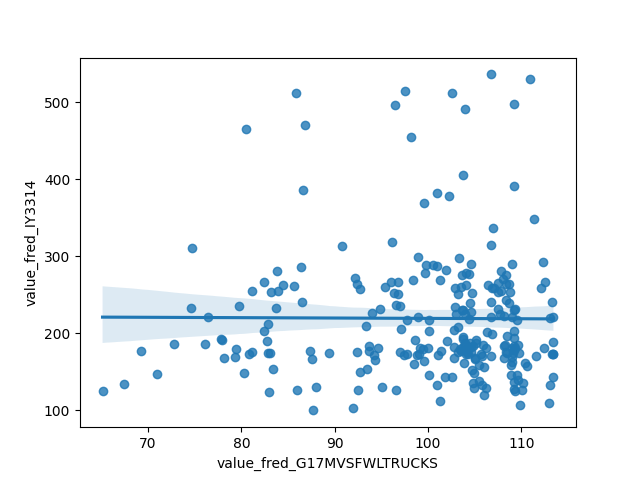
\includegraphics[scale = 0.9]{plots/plot_2026-10-19.png}
\caption{Raw Regression Plot for 2026-10-19}
\end{figure}
\newpage
\subsection{Detrended Regression}
\noindent Regresses the residuals of each series after removing its own linear time trend, so a shared trend can no longer drive the result on its own. A relationship that stays significant here is better evidence of a genuine link between the two series.

\begin{center}
\begin{tabular}{lclc}
\toprule
\textbf{Dep. Variable:}                          & value\_fred\_IY3314\_detrended & \textbf{  R-squared:         } &     0.000   \\
\textbf{Model:}                                  &              OLS               & \textbf{  Adj. R-squared:    } &    -0.004   \\
\textbf{Method:}                                 &         Least Squares          & \textbf{  F-statistic:       } &   0.02068   \\
\textbf{Date:}                                   &        Mon, 19 Oct 2026        & \textbf{  Prob (F-statistic):} &    0.886    \\
\textbf{Time:}                                   &            17:51:42            & \textbf{  Log-Likelihood:    } &   -1346.8   \\
\textbf{No. Observations:}                       &                249             & \textbf{  AIC:               } &     2698.   \\
\textbf{Df Residuals:}                           &                247             & \textbf{  BIC:               } &     2705.   \\
\textbf{Df Model:}                               &                  1             & \textbf{                     } &             \\
\textbf{Covariance Type:}                        &           nonrobust            & \textbf{                     } &             \\
\bottomrule
\end{tabular}
\begin{tabular}{lcccccc}
                                                 & \textbf{coef} & \textbf{std err} & \textbf{t} & \textbf{P$> |$t$|$} & \textbf{[0.025} & \textbf{0.975]}  \\
\midrule
\textbf{const}                                   &   -6.754e-12  &        3.439     & -1.96e-12  &         1.000        &       -6.774    &        6.774     \\
\textbf{value\_fred\_G17MVSFWLTRUCKS\_detrended} &       0.0475  &        0.330     &     0.144  &         0.886        &       -0.603    &        0.697     \\
\bottomrule
\end{tabular}
\begin{tabular}{lclc}
\textbf{Omnibus:}       & 75.189 & \textbf{  Durbin-Watson:     } &    0.024  \\
\textbf{Prob(Omnibus):} &  0.000 & \textbf{  Jarque-Bera (JB):  } &  174.874  \\
\textbf{Skew:}          &  1.427 & \textbf{  Prob(JB):          } & 1.06e-38  \\
\textbf{Kurtosis:}      &  5.952 & \textbf{  Cond. No.          } &     10.4  \\
\bottomrule
\end{tabular}
%\caption{OLS Regression Results}
\end{center}

Notes: \newline
 [1] Standard Errors assume that the covariance matrix of the errors is correctly specified.

\begin{figure}
\centering
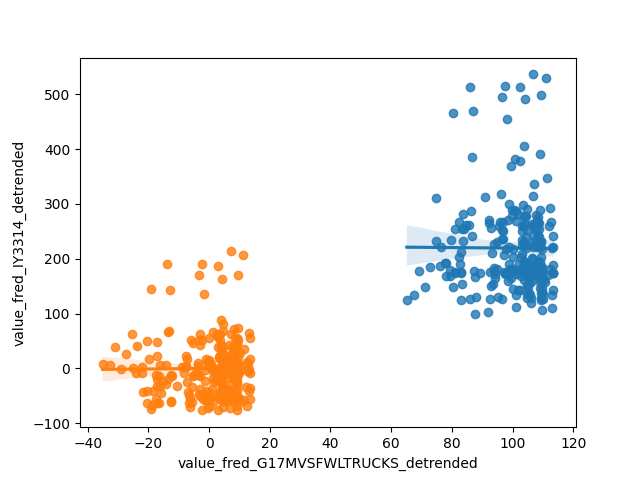
\includegraphics[scale = 0.9]{plots/plot_2026-10-19_detrended.png}
\caption{Detrended Regression Plot for 2026-10-19}
\end{figure}
\newpage
